\chapter{Design Phase}

\section{Explain and Design the Entity Class Diagram}

\subsection{Add ID Attributes to Entity Classes}

None of the entity classes inherits from another class, so the attribute ID: int is added to all entity classes. This identifier is necessary because each object must be uniquely distinguished when the system stores and retrieves data.

The class User has ID: int to identify each staff account. The class Restaurant has ID: int to identify each restaurant in the restaurant chain. The class Employee has ID: int to identify each part-time employee. The class Shift has ID: int to identify each working shift. The class RegistrationShift has ID: int to identify each registration record created when an employee registers for a shift.

\subsection{Add Types for All Attributes}


In User, the attributes username, password, role, and description are designed as String values. In Restaurant, the attributes restaurantName, address, and description are also String values. In Employee, the attributes code, phoneNumber, fullName, and email are String values, while dob and contractDate are Date values. In Shift, the working day is represented by date: Date, the shift order is represented by shiftNumber: int, and the time range is represented by startDate: Date and endDate: Date. In RegistrationShift, registeredTime is designed as DateTime, while status and description are String values.

\subsection{Convert Association Relationships to Aggregation or \\ Composition Relationships}




The association relationship that needs to be converted in this part is the relationship in which Employee and Shift are linked through RegistrationShift. This relationship represents the fact that one employee can register for many shifts, and one shift can be registered by many employees. Therefore, RegistrationShift is used as the object that records each concrete registration between one employee and one shift.

This association is converted into aggregation relationships in the design entity class diagram. First, RegistrationShift aggregates Employee, because each registration record refers to one selected employee, while the employee object can still exist independently from the registration record. Second, RegistrationShift aggregates Shift, because each registration record refers to one selected shift, while the shift object can also exist independently. Third, RegistrationShift aggregates User, because each registration record must keep the staff account that created it, but the user account is not owned by the registration record. In the design entity class diagram, these three relationships are represented by white diamonds at RegistrationShift.


\subsection{Add Object Attributes Based on Aggregation and \\ Composition Relationships}


Employee is a component of Restaurant, with a 1--n relationship from Restaurant to Employee. Therefore, Restaurant has a list of employees, represented by the object attribute employees: Employee[].

RegistrationShift aggregates Employee, with a 1--n relationship from Employee to RegistrationShift. Therefore, each RegistrationShift has one employee, represented by the object attribute employee: Employee.

RegistrationShift aggregates Shift, with a 1--n relationship from Shift to RegistrationShift. Therefore, each RegistrationShift has one shift, represented by the object attribute shift: Shift.

RegistrationShift aggregates User, with a 1--n relationship from User to RegistrationShift. Therefore, each RegistrationShift has one user, represented by the object attribute user: User. This attribute records which registration staff created the shift registration.

As a result, the Design Phase entity class diagram contains the same core entity classes as the Analysis Phase, but each class is now more concrete and implementation-oriented. The diagram includes identifiers, typed attributes, and object attributes that represent the aggregation and composition relationships among the classes.

\begin{figure}[H]
    \centering
    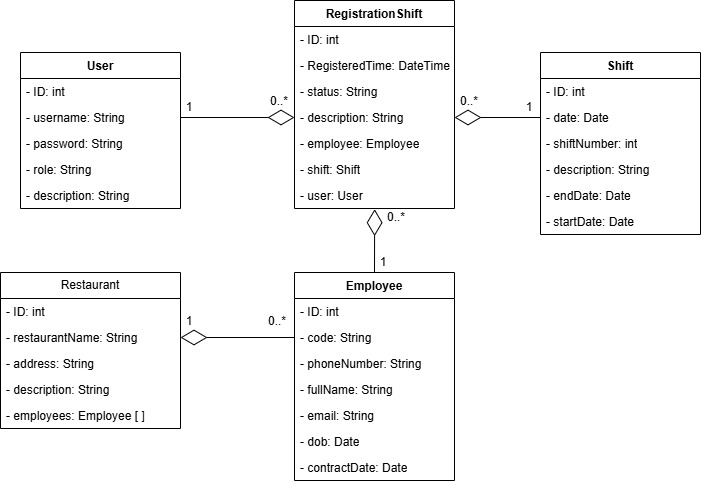
\includegraphics[width=0.9\textwidth]{assets/diagrams/Entity Class - Design.jpg}
    \caption{Entity Class Diagram in the Design Phase}
\end{figure}
\section{Explain and Design the Database Diagram}

\subsection{Create Tables from Entity Classes}

The entity class User is mapped to the table tblUser, which stores the registration staff accounts used to log in and perform the registration operation. The entity class Restaurant is mapped to the table tblRestaurant, which stores restaurant information in the restaurant chain. The entity class Employee is mapped to the table tblEmployee, which stores the information of part-time employees. The entity class Shift is mapped to the table tblShift, which stores the working shifts of each day. Finally, the entity class RegistrationShift is mapped to the table tblRegistrationShift, which stores each registration record between an employee and a shift.

\subsection{Transfer Non-Object Attributes to Table Columns}


For tblUser, the columns are ID, username, password, role, and description. For tblRestaurant, the columns are ID, restaurantName, address, and description. For tblEmployee, the columns are ID, code, fullName, phoneNumber, email, dob, and contractDate. For tblShift, the columns are ID, date, shiftNumber, description, startDate, and endDate. For tblRegistrationShift, the non-object columns are ID, registeredTime, status, and description; the relationships to Employee, Shift, and User are represented by foreign keys.


\subsection{Configure Primary Keys and Foreign Keys}

For primary keys, every table has the column ID, so this column is configured as the primary key of its table. Therefore, tblUser.ID, tblRestaurant.ID, tblEmployee.ID, tblShift.ID, and tblRegistrationShift.ID are the primary keys of the five tables.

For foreign keys, since one tblRestaurant can have many tblEmployee records, tblEmployee contains the foreign key restaurantID, which references tblRestaurant.ID. Since one tblEmployee can appear in many registration records, tblRegistrationShift contains the foreign key employeeID, which references tblEmployee.ID. Since one tblShift can appear in many registration records, tblRegistrationShift contains the foreign key shiftID, which references tblShift.ID. Since one tblUser can create many registration records, tblRegistrationShift contains the foreign key userID, which references tblUser.ID.

As a result, the final database design contains five tables. tblUser stores staff account data with text fields such as username, password, role, and description. tblRestaurant stores restaurant information with restaurantName, address, and description. tblEmployee stores employee information and includes restaurantID as a foreign key. tblShift stores shift information, including the date, shift number, description, start date, and end date. tblRegistrationShift stores registration records and includes employeeID, shiftID, and userID as foreign keys. This design ensures that the database can store the registration data while preserving the relationships among employees, shifts, restaurants, and registration staff.

\begin{figure}[H]
    \centering
    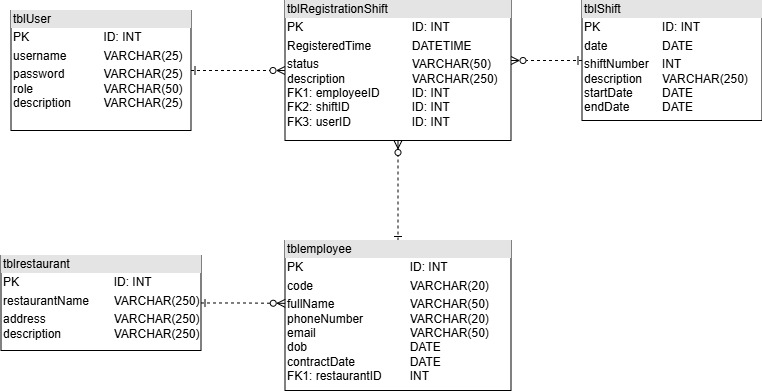
\includegraphics[width=0.95\textwidth]{assets/diagrams/Database - Design.jpg}
    \caption{Database Diagram in the Design Phase}
\end{figure}
\section{Design the Interfaces}


The module contains four main interface classes: LoginFrm, HomeFrm, SearchEmployeeFrm, and RegisterShiftFrm. These interfaces are arranged according to the working flow of the registration staff: login, choose the registration function, search for an employee, and register next week's shifts for the selected employee.

\subsection{Login Interface - LoginFrm}

LoginFrm is the first interface of the application. Its main purpose is to allow the registration staff to enter authentication information before accessing the system. The interface contains two input fields: one field for the username and one field for the password. The username field is used to identify the staff account, while the password field is used to verify that the person logging in is authorized to use the system.

The interface also contains a \textit{Login} button. After the registration staff enters the username and password, this button is used to submit the login information to the system. If the login information is correct, the system continues to the staff homepage. If the login information is incorrect, the system should display an error message and remain on the login screen. Since this is the first interface in the flow, it does not receive any hidden data from a previous screen.

\begin{figure}[H]
    \centering
    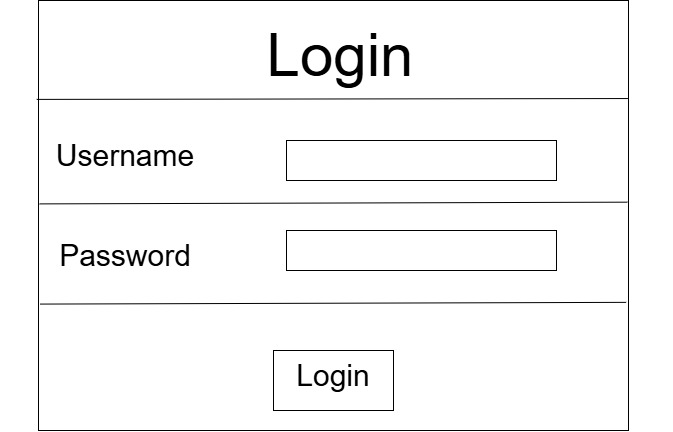
\includegraphics[width=0.75\textwidth]{assets/diagrams/Login Interface.jpg}
    \caption{Login Interface for Registration Staff}
\end{figure}

\subsection{Staff Home Interface - HomeFrm}

HomeFrm is the staff homepage displayed after a successful login. This interface represents the starting point for the registration staff after entering the system. In the context of Module 1, the homepage provides access to the function for registering next week's shifts.

The main control on this interface is the \textit{Register for next week} button. When the registration staff chooses this button, the system opens the employee search interface. The homepage may also display information about the currently logged-in staff, such as the staff name, so that the system clearly shows which user is operating the module. 

\begin{figure}[H]
    \centering
    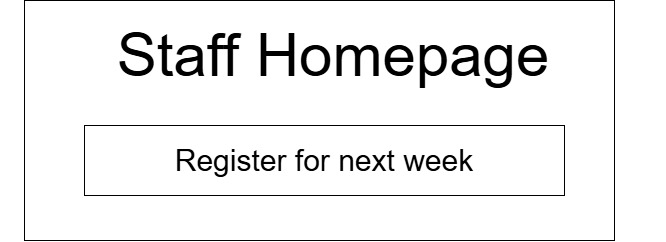
\includegraphics[width=0.75\textwidth]{assets/diagrams/Hompage Interface.jpg}
    \caption{Staff Home Interface for the Register Next Week Function}
\end{figure}

\subsection{Search Employee Interface - SearchEmployeeFrm}

SearchEmployeeFrm is the interface used to search for the part-time employee who requests next week's shift registration. This interface appears after the registration staff selects the Register for next week function from the homepage.

The interface contains an input field for entering the employee name keyword. The registration staff uses this field to type part or all of the employee's name. Next to the input field, there is a \textit{Search} button. When this button is clicked, the system searches for employees whose names match the entered keyword.

The search results are displayed in a table. The table shows the main information needed for the staff to identify the correct employee, including the ordinal number, employee code, employee name, and phone number. The table also provides a selection column, allowing the staff to choose the correct employee from the result list. This design is necessary because more than one employee may have a similar name, so the staff must be able to compare the employee code and phone number before selecting one employee.


\begin{figure}[H]
    \centering
    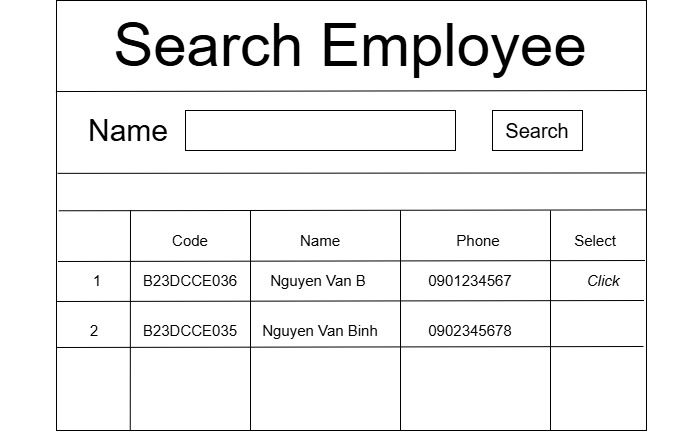
\includegraphics[width=0.85\textwidth]{assets/diagrams/Search Employee Interface.jpg}
    \caption{Search Employee Interface}
\end{figure}

\subsection{Register Next Week's Shift Interface - RegisterShiftFrm}

RegisterShiftFrm is the main interface for registering next week's shifts for the selected employee. This interface appears after the registration staff selects the correct employee from the search result table.

At the top of the interface, the system displays the selected employee's information, including employee code, employee name, and phone number. This information is read-only and helps the staff confirm that the registration is being performed for the correct employee before selecting any shifts.

The central part of the interface is a shift registration table. The table is organized by the seven days of the next week, from Monday to Sunday. For each day, there are two shift columns: Shift 1 from 8am to 4pm and Shift 2 from 4pm to 12am. Each shift cell contains a checkbox. The registration staff ticks the checkboxes corresponding to the shifts that the employee wants to register. This table is both an output area and an input area: it displays the available shift structure of the next week, and it also receives the staff's selected shift choices.

At the bottom of the interface, the \textit{Save} button is used to submit the selected shifts. When the staff clicks this button, the system counts the selected checkboxes, checks whether the total number of registered shifts satisfies the minimum threshold, creates the corresponding registration records, and saves them into the database. If the selected number of shifts is not enough, the system should show an error message. If the save operation is successful, the system displays a success message and returns to the appropriate next screen in the registration flow.


\begin{figure}[H]
    \centering
    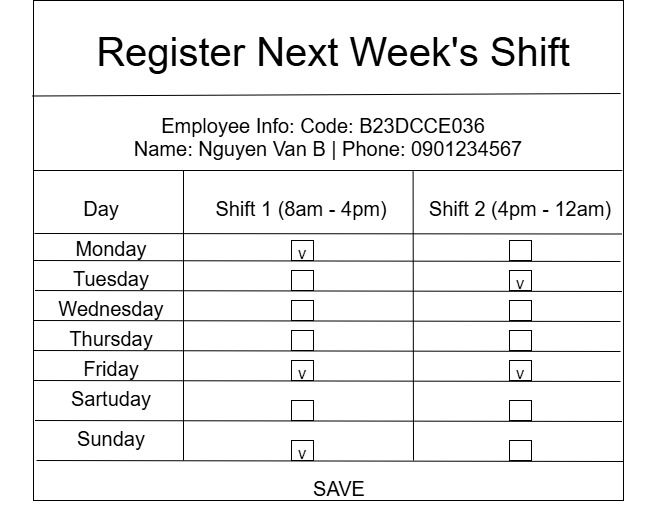
\includegraphics[width=0.85\textwidth]{assets/diagrams/Register Next Week's Shift Interface.jpg}
    \caption{Register Next Week's Shift Interface}
\end{figure}

\section{Explain and Design the Full Class Diagram}


\subsection{Design View Classes as Boundary Classes}

The View layer contains the boundary classes that correspond to the interfaces in the module. Each form class inherits from JFrame because it is a window-based interface. Each form also implements ActionListener so that it can receive and handle user actions such as clicking a button or selecting a table row.

\subsubsection{LoginFrm}

LoginFrm is the first boundary class of the module. It is responsible for receiving the login information of the registration staff. The explicit attributes of this class are txtUserName: JTextField, txtPassword: JTextField, and btnLogin: JButton. The username text field receives the staff username, the password text field receives the password, and the login button submits the authentication request.

This form has no hidden attribute because it is the first screen of the application flow and does not receive any object from a previous form. Therefore, its constructor is LoginFrm() with no parameter. The method actionPerformed(e: ActionEvent): void receives events from the form, and btnLoginClick(): void handles the login button. In this method, the form gets the username and password, creates a User object for authentication data, and calls UserDAO.checkLogin(user: User): boolean. If the login is successful, the system opens HomeFrm and passes the authenticated User object forward.

\subsubsection{HomeFrm}

HomeFrm is the staff home interface after successful login. Its explicit attribute is btnRegister: JButton, which allows the registration staff to choose the function \textit{Register for next week}. The hidden attribute is user: User. This object is passed from LoginFrm and represents the currently logged-in staff member.

Because HomeFrm needs to remember the authenticated staff, its constructor is HomeFrm(u: User). The method actionPerformed(e: ActionEvent): void dispatches form events, while btnRegisterClick(): void handles the event when the staff chooses the registration function. After this button is clicked, the system opens SearchEmployeeFrm and passes the same User object to the next form.

\subsubsection{SearchEmployeeFrm}

SearchEmployeeFrm is the boundary class used to search for the employee who wants to register next week's shifts. Its explicit attributes are txtName: JTextField, btnSearch: JButton, and tblResult: JTable. The text field receives the employee name keyword, the search button submits the search request, and the result table displays the matched employees so that the staff can select the correct employee.

The hidden attribute of this form is user: User, which is received from HomeFrm. This attribute is not the main displayed data of the search interface, but it must be kept because the selected employee and the logged-in user will both be needed in the next registration form. Therefore, the constructor is SearchEmployeeFrm(u: User). The method btnSearchClick(): void gets the keyword from txtName, calls EmployeeDAO.searchEmployee(key: String): ArrayList<Employee>, and displays the returned employee list in tblResult. The method btnResultClick(): void handles the event when the staff selects one employee from the result table, then opens RegisterShiftFrm with the selected Employee object and the hidden User object.

\subsubsection{RegisterShiftFrm}

RegisterShiftFrm is the main boundary class for registering next week's shifts. Its explicit attributes are tblShift: JTable and btnSave: JButton. The shift table displays the available shifts of the next week and allows the staff to select the shifts requested by the employee. The save button submits the selected shifts to the system.

This form has two hidden attributes: employee: Employee and user: User. The employee object is the selected employee from SearchEmployeeFrm; it is used to create registration records for the correct employee. The user object is the logged-in staff member; it is used to record who performs the registration. Therefore, the constructor is RegisterShiftFrm(e: Employee, u: User). During initialization, this form calls ShiftDAO.getShiftNextWeek(): ArrayList<Shift> to load next week's shifts and calls \\ RegistrationShiftDAO.getRegistrationByEmployee(e: Employee): ArrayList<RegistrationShift> to get existing registrations of the selected employee. The method btnSaveClick(): void collects the selected shifts, creates a list of RegistrationShift objects, and calls RegistrationShiftDAO.saveRegistration(list: \\ ArrayList<RegistrationShift>): boolean to save the data.

\subsection{Design DAO Classes as Control/Data Access Classes}



\subsubsection{Operation: Check Login - checkLogin}

This operation is triggered at LoginFrm through btnLoginClick(). Its purpose is to verify whether the login credentials entered by the registration staff are correct.

The input data consists of username: String and password: String. There are two input parameter candidates. The first candidate is checkLogin(String username, String password), which passes the two fields separately. The second candidate is checkLogin(User u), which passes a User object containing the username and password. The selected design is checkLogin(User u), because encapsulating related account data into a single User object is cleaner and more maintainable.

The output needs to convey whether login is correct and also allow the system to know the staff role after login. There are three output candidates: boolean, String, and User. Returning String only provides the role or description and does not clearly express success or failure. Returning User can contain full information, but the instructor's sample diagrams commonly use boolean for login checking. Therefore, the selected output is boolean. In Java, objects are passed by reference, so the DAO method can populate the User object's fields, such as role and description, when a matching account is found, then return true or false as the login result.

The output is boolean, which is a primitive type and has no corresponding DAO class. Therefore, the assignment is based on the input object. Since the input object is User, this operation is assigned to UserDAO. The final signature is checkLogin(User u): boolean.

\subsubsection{Operation: Search Employee - searchEmployee}

This operation is triggered at SearchEmployeeFrm through btnSearchClick(). Its purpose is to search all employees whose fullName contains the keyword entered by the registration staff.

The input data is the search keyword. There are two input parameter candidates. The first candidate is searchEmployee(String key), which passes the keyword directly as a string. The second candidate is searchEmployee(Employee e), which passes an Employee object with the name field set. Since the input is only a simple keyword and not a full Employee object, the selected design is searchEmployee(String key).

The output is a list of Employee objects matching the keyword. There are four output candidates: Employee[], List<Employee>, Vector<Employee>, and ArrayList<Employee>. The array option is eliminated because it is fixed-size and inconvenient for dynamic search results. Vector<Employee> is eliminated because it is a legacy collection and has unnecessary overhead for this case. Between List<Employee> and ArrayList<Employee>, the selected design is ArrayList<Employee>, because it matches the concrete collection style used in the design diagram and in the instructor's sample pattern.

The output is ArrayList<Employee>, which is related to Employee. Therefore, this operation is assigned to EmployeeDAO. The final signature is searchEmployee(String key): ArrayList<Employee>.

\subsubsection{Operation: Get Shifts for Next Week - getShiftNextWeek}

This operation is triggered at RegisterShiftFrm during form initialization. Its purpose is to load the fourteen shifts of the next week for the seven-day and two-shift registration table.

For the input parameter, there are two candidates. The first candidate is getShiftNextWeek(), where the method calculates the next week's date range internally. The second candidate is getShiftNextWeek(Date startDate), where the start date of next week is passed from outside. The selected design is getShiftNextWeek(), because the next week can be determined by the system and the form does not need to calculate and pass this value.

The output is a list of Shift objects for the next week. The output candidates are Shift[] and ArrayList<Shift>. The array option is less convenient for database query results, so the selected output is ArrayList<Shift>.

The output is ArrayList<Shift>, which is related to Shift. Therefore, this operation is assigned to ShiftDAO. The final signature is getShiftNextWeek(): ArrayList<Shift>.

\subsubsection{Operation: Save Registration - saveRegistration}

This operation is triggered at RegisterShiftFrm through btnSaveClick(). Its purpose is to save all shift registrations selected for an employee into the database.

The input data consists of multiple RegistrationShift records. Each record contains employee, shift, user, registeredTime, and status. There are three input parameter candidates. The first candidate is saveRegistration(Employee e, Shift s, User u), which passes individual objects for each selected shift. This option is eliminated because it is not object-oriented enough and does not represent the registration as a separate domain object. The second candidate is saveRegistration(RegistrationShift rs), which passes one RegistrationShift object. This option is possible, but it requires the method to be called many times when the employee selects many shifts. The third candidate is saveRegistration(ArrayList<RegistrationShift> list), which passes all registration records at once. This option is selected because it supports saving all selected shifts in one call and is suitable for batch database operations.

The output needs to convey whether the save operation succeeded or failed. There are three output candidates: void, boolean, and int. The void option is eliminated because it gives no feedback to the caller. The int option can return the number of records saved, but this is more detailed than required by the interface. Therefore, the selected output is boolean, because it is simple and sufficient for displaying a success or failure message.

The output is boolean, which is a primitive type. Therefore, the DAO assignment is based on the input entity. Since the input is ArrayList<RegistrationShift>, this operation is assigned to RegistrationShiftDAO. The final signature is RegistrationShiftDAO.saveRegistration(ArrayList<RegistrationShift> list): boolean.

\subsubsection{Operation: Get Registration by Employee - getRegistrationByEmployee}

This operation is triggered at RegisterShiftFrm during form initialization. Its purpose is to retrieve all existing shift registrations of the selected employee for the next week.

The input is the employee whose registration records need to be retrieved. There are two input parameter candidates. The first candidate is getRegistrationByEmployee(int employeeID), which passes only the employee's ID. The second candidate is getRegistrationByEmployee(Employee e), which passes the Employee object. The selected design is getRegistrationByEmployee(Employee e), because it follows the object-oriented approach and is consistent with the way the selected Employee object is passed between forms.

The output is a list of RegistrationShift records for the employee. The output candidates are RegistrationShift[] and ArrayList<RegistrationShift>. The array option is eliminated because the number of registration records may vary. The selected output is ArrayList<RegistrationShift>, which is suitable for a dynamic list of records.

The output is ArrayList<RegistrationShift>, which is related to RegistrationShift. Therefore, this operation is assigned to RegistrationShiftDAO. The final signature is getRegistrationByEmployee(Employee e): ArrayList<RegistrationShift>.

\subsection{Present Entity Classes in the Model Layer}

The entity classes form the Model layer of the design. User represents the staff account that logs in and performs the registration operation. Its attributes include ID: int, username: String, password: String, role: String, and description: String.

Restaurant represents a restaurant in the restaurant chain. Its attributes include ID: int, restaurantName: String, address: String, description: String, and the object attribute employees: Employee[]. This object attribute represents the list of employees managed by the restaurant.

Employee represents a part-time employee whose shifts can be registered. Its attributes include ID: int, code: String, phoneNumber: String, fullName: String, email: String, dob: Date, and contractDate: Date.

Shift represents one working shift. Its attributes include ID: int, date: Date, shiftNumber: int, description: String, startDate: Date, and endDate: Date.

RegistrationShift represents a registration record that connects one employee with one selected shift and the staff member who creates the record. Its attributes include ID: int, registeredTime: DateTime, status: String, and description: String. It also has the object attributes employee: Employee, shift: Shift, and user: User.

\subsection{Summary of View, DAO, and Entity Classes}

This part summarizes the three main groups of classes in the full class diagram: View classes, Control/DAO classes, and Entity classes. These groups show how the module follows the MVC-oriented design structure.

\subsubsection{View Classes}

LoginFrm is the interface to login. It needs a text field to enter the username, a text field to enter the password, and a button to login.

HomeFrm is the home interface for the Registration Staff. It needs at least a button to go to the Register for next week function. It also displays the logged-in staff's name via a label.

SearchEmployeeFrm is the interface to search the employee to register shifts for. It needs a text field to enter the keyword to search employee by name, a button to search, and a table to show the list of matched employees.

RegisterShiftFrm is the interface to register shifts for the selected employee. It needs a label to display the selected employee's information, including code, name, and phone. It also needs a table with seven rows for the seven days of next week and two columns for Shift 1 and Shift 2 containing checkboxes, and a button to save the registration.

\subsubsection{Control Classes: DAO --- Data Access Object}

DAO is the general abstract class of DAO. It has only the attribute con: Connection and the constructor DAO() to connect to the database. It provides the common connection for all inherited DAO classes in the system.

UserDAO is the class for manipulating the database related to the User object. In this module, it needs one method: checkLogin(User u): boolean. This method verifies whether the login information is correct. If the credentials match a record in the database, the User object's fields, such as ID, role, and description, are populated and the method returns true. Otherwise, it returns false.

EmployeeDAO is the class for manipulating the database related to the Employee object. In this module, it needs one method: searchEmployee(String key): ArrayList<Employee>. This method searches all employees whose fullName contains the entered keyword.

ShiftDAO is the class for manipulating the database related to the Shift object. In this module, it needs one method: getShiftNextWeek(): ArrayList<Shift>. This method retrieves all fourteen shifts of the next week from the database.

RegistrationShiftDAO is the class for manipulating the database related to the RegistrationShift object. In this module, it needs two methods. The first method is saveRegistration(ArrayList<RegistrationShift> list): boolean, which saves all shift registrations for an employee into the database in a batch operation. The second method is getRegistrationByEmployee(Employee e): ArrayList<RegistrationShift>, which retrieves all existing registrations of a given employee for the next week and is used to pre-populate the checkbox table.

\subsubsection{Entity Classes}

User represents the system user or staff who operates the application. Its attributes include ID: int, username: String, password: String, role: String, and description: String.

Employee represents the part-time employee whose shifts are being registered. Its attributes include ID: int, code: String, fullName: String, phoneNumber: String, email: String, dob: Date, and contractDate: Date.

Shift represents a working shift in the schedule. Its attributes include ID: int, date: Date, shiftNumber: int, description: String, startDate: Date, and endDate: Date.

RegistrationShift represents a shift registration record linking an employee to a shift. Its attributes include ID: int, registeredTime: DateTime, status: String, and description: String. It has aggregation relationships with Employee as the registered employee, Shift as the selected shift, and User as the staff who created the registration.

Restaurant represents the restaurant where employees work. Its attributes include ID: int, restaurantName: String, address: String, and description: String. It has a one-to-many relationship with Employee.

\subsection{Explain the Main Relationships in the Full Class Diagram}

In the View layer, all form classes inherit from JFrame and implement ActionListener. This shows that the forms are graphical windows and can handle user events. The navigation relationships follow the standard flow of the module: LoginFrm opens HomeFrm, HomeFrm opens SearchEmployeeFrm, and SearchEmployeeFrm opens RegisterShiftFrm.

The View classes connect to DAO classes only when they need database operations. LoginFrm uses UserDAO to check login information. SearchEmployeeFrm uses EmployeeDAO to search employees. RegisterShiftFrm uses ShiftDAO to load next week's shifts and uses RegistrationShiftDAO to retrieve and save registration records.

The DAO classes inherit from DAO, so they share the common database connection. Each specific DAO class manipulates the database data related to its corresponding entity class: UserDAO works with User, EmployeeDAO works with Employee, ShiftDAO works with Shift, and RegistrationShiftDAO works with RegistrationShift.

In the Entity layer, Restaurant has a composition relationship with Employee, because a restaurant manages many employees. RegistrationShift has aggregation relationships with Employee, Shift, and User. Each registration record refers to one selected employee, one selected shift, and one staff account that created the registration, while these three objects can still exist independently from the registration record.

\begin{figure}[H]
    \centering
    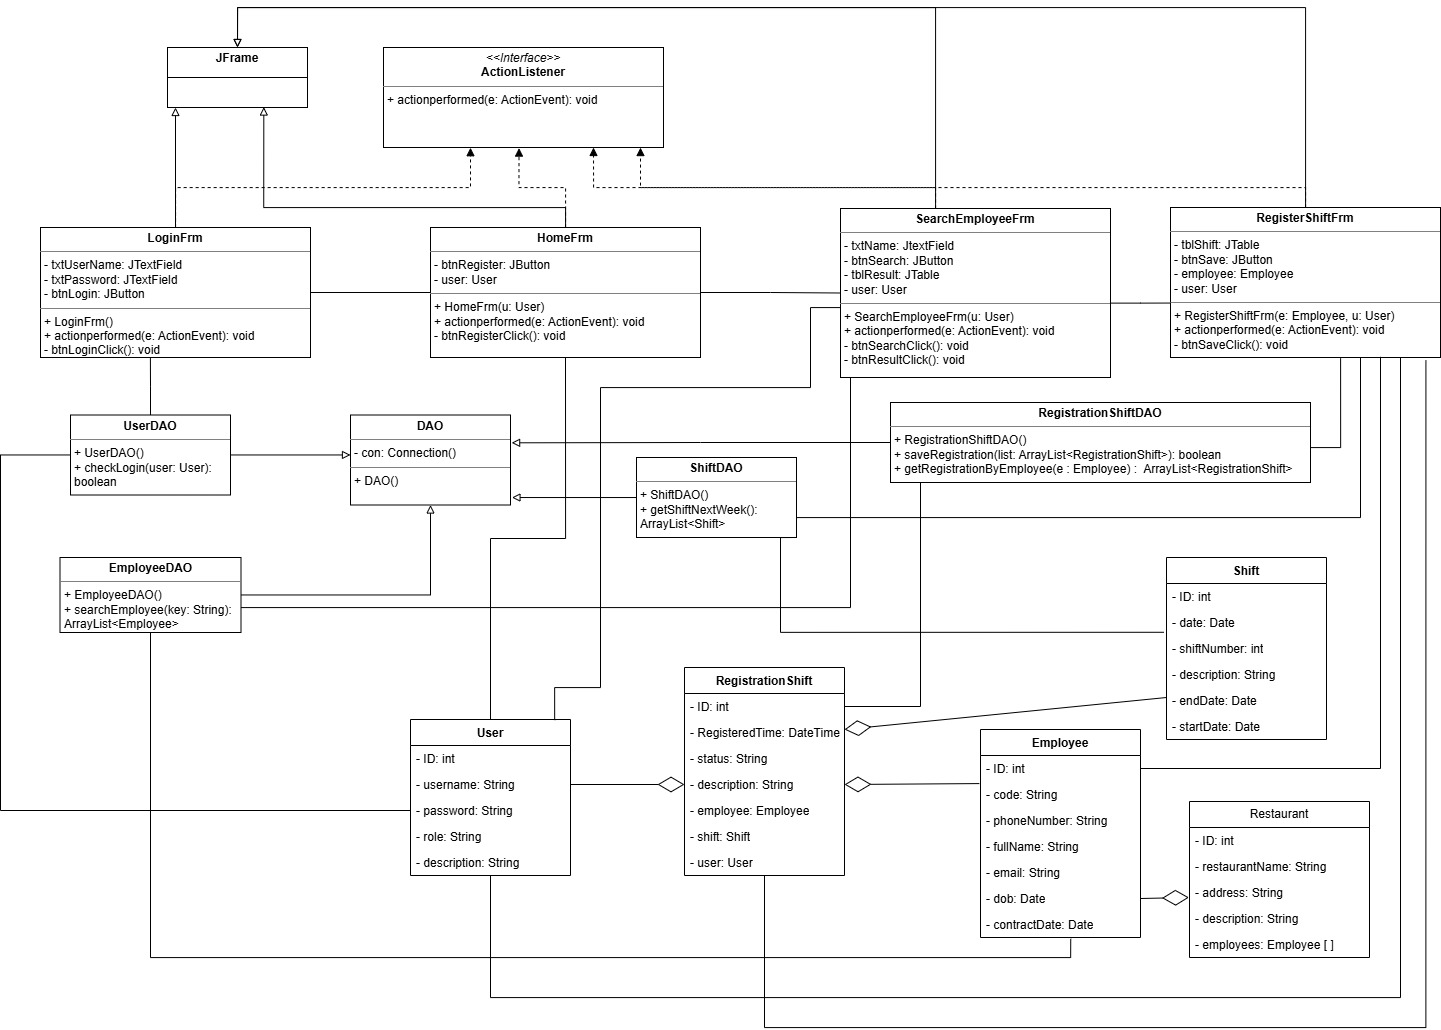
\includegraphics[width=0.95\textwidth]{assets/diagrams/Classes Diagram Design.jpg}
    \caption{Full Class Diagram in the Design Phase}
\end{figure}

\section{Scenario v.3 and the Sequence Diagram for the Standard Scenario of the Module}


\subsection{Scenario v.3 for the Standard Scenario}

\begin{enumerate}
    \item A part-time employee comes to the restaurant and requests the registration staff to register his available shifts for the next week.
    \item The registration staff enters his username and password, then clicks the Login button on LoginFrm.
    \item The method actionPerformed() of LoginFrm is called.
    \item The method actionPerformed() calls the class User to create a User object.
    \item The class User packs the username and password into a User object.
    \item The class User returns the User object to the method actionPerformed().
    \item The method actionPerformed() calls the method checkLogin() of the class UserDAO.
    \item The method checkLogin() checks the login information against the database.
    \item The method checkLogin() calls the class User to set more user attributes, such as role and description.
    \item The class User calls its setter methods setRole() and setDescription().
    \item The class User returns the updated User object to the method checkLogin().
    \item The method checkLogin() returns the login result as a boolean value to the method actionPerformed().
    \item The method actionPerformed() calls the class HomeFrm.
    \item The constructor HomeFrm(u: User) is called.
    \item The interface HomeFrm is shown to the registration staff.
    \item The registration staff clicks the Register for next week button.
    \item The method actionPerformed() of HomeFrm is called.
    \item The method actionPerformed() calls the class SearchEmployeeFrm.
    \item The constructor SearchEmployeeFrm(u: User) is called.
    \item The interface SearchEmployeeFrm is shown to the registration staff.
    \item The registration staff asks the part-time employee for his name.
    \item The part-time employee provides his name to the registration staff.
    \item The registration staff enters the employee name keyword and clicks the Search button.
    \item The method actionPerformed() of SearchEmployeeFrm is called.
    \item The method actionPerformed() calls the method searchEmployee() of the class EmployeeDAO.
    \item The method searchEmployee() executes the employee search operation.
    \item The method searchEmployee() calls the class Employee to pack the search results.
    \item The class Employee packs each result into an Employee object.
    \item The class Employee returns the Employee objects to the method searchEmployee().
    \item The method searchEmployee() returns the employee results to the method actionPerformed().
    \item The method actionPerformed() displays the results on SearchEmployeeFrm to the registration staff.
    \item The registration staff clicks the correct employee in the result list.
    \item The method actionPerformed() of SearchEmployeeFrm is called.
    \item The method actionPerformed() calls the class RegisterShiftFrm.
    \item The constructor RegisterShiftFrm(e: Employee, u: User) is called.
    \item The constructor RegisterShiftFrm(e: Employee, u: User) calls the method getShiftNextWeek() of the class ShiftDAO.
    \item The method getShiftNextWeek() of the class ShiftDAO is called.
    \item The method getShiftNextWeek() calls the class Shift to pack the results.
    \item The constructor Shift() is called.
    \item The class Shift returns the Shift objects to the method getShiftNextWeek().
    \item The method getShiftNextWeek() returns the shift results to the constructor RegisterShiftFrm(e: Employee, u: User).
    \item The interface RegisterShiftFrm is shown to the registration staff with the employee information and the $7 \times 2$ shift registration table.
    \item The registration staff asks the part-time employee which shifts he wants to work next week.
    \item The part-time employee provides his desired shifts to the registration staff.
    \item The registration staff ticks the corresponding checkboxes and clicks the Save button.
    \item The method actionPerformed() of RegisterShiftFrm is called.
    \item The method actionPerformed() calls the class RegistrationShift to pack the registration data.
    \item The constructor RegistrationShift() is called.
    \item The class RegistrationShift returns the list of RegistrationShift objects to the method actionPerformed().
    \item The method actionPerformed() calls the method saveRegistration() of the class RegistrationShiftDAO.
    \item The method saveRegistration() of the class RegistrationShiftDAO is called.
    \item The method saveRegistration() returns the save result to the method actionPerformed().
    \item The method actionPerformed() displays a success message to the registration staff.
    \item The registration staff informs the part-time employee that the registration is successful.
    \item The registration staff clicks the OK button of the message.
    \item The method actionPerformed() of RegisterShiftFrm is called.
    \item The method actionPerformed() calls the class HomeFrm.
    \item The interface HomeFrm is shown to the registration staff.
\end{enumerate}


After the correct employee is selected, SearchEmployeeFrm opens RegisterShiftFrm with the selected Employee object and the logged-in User object. During the constructor execution, RegisterShiftFrm calls ShiftDAO.getShiftNextWeek() to load the next week's shifts and display the registration table. The staff then selects the shifts requested by the employee. For each selected shift, the system creates a RegistrationShift object containing the employee, shift, user, registered time, and status. Finally, RegisterShiftFrm calls RegistrationShiftDAO.saveRegistration() to save the registration data, displays a success message, and returns to HomeFrm.

\begin{figure}[H]
    \centering
    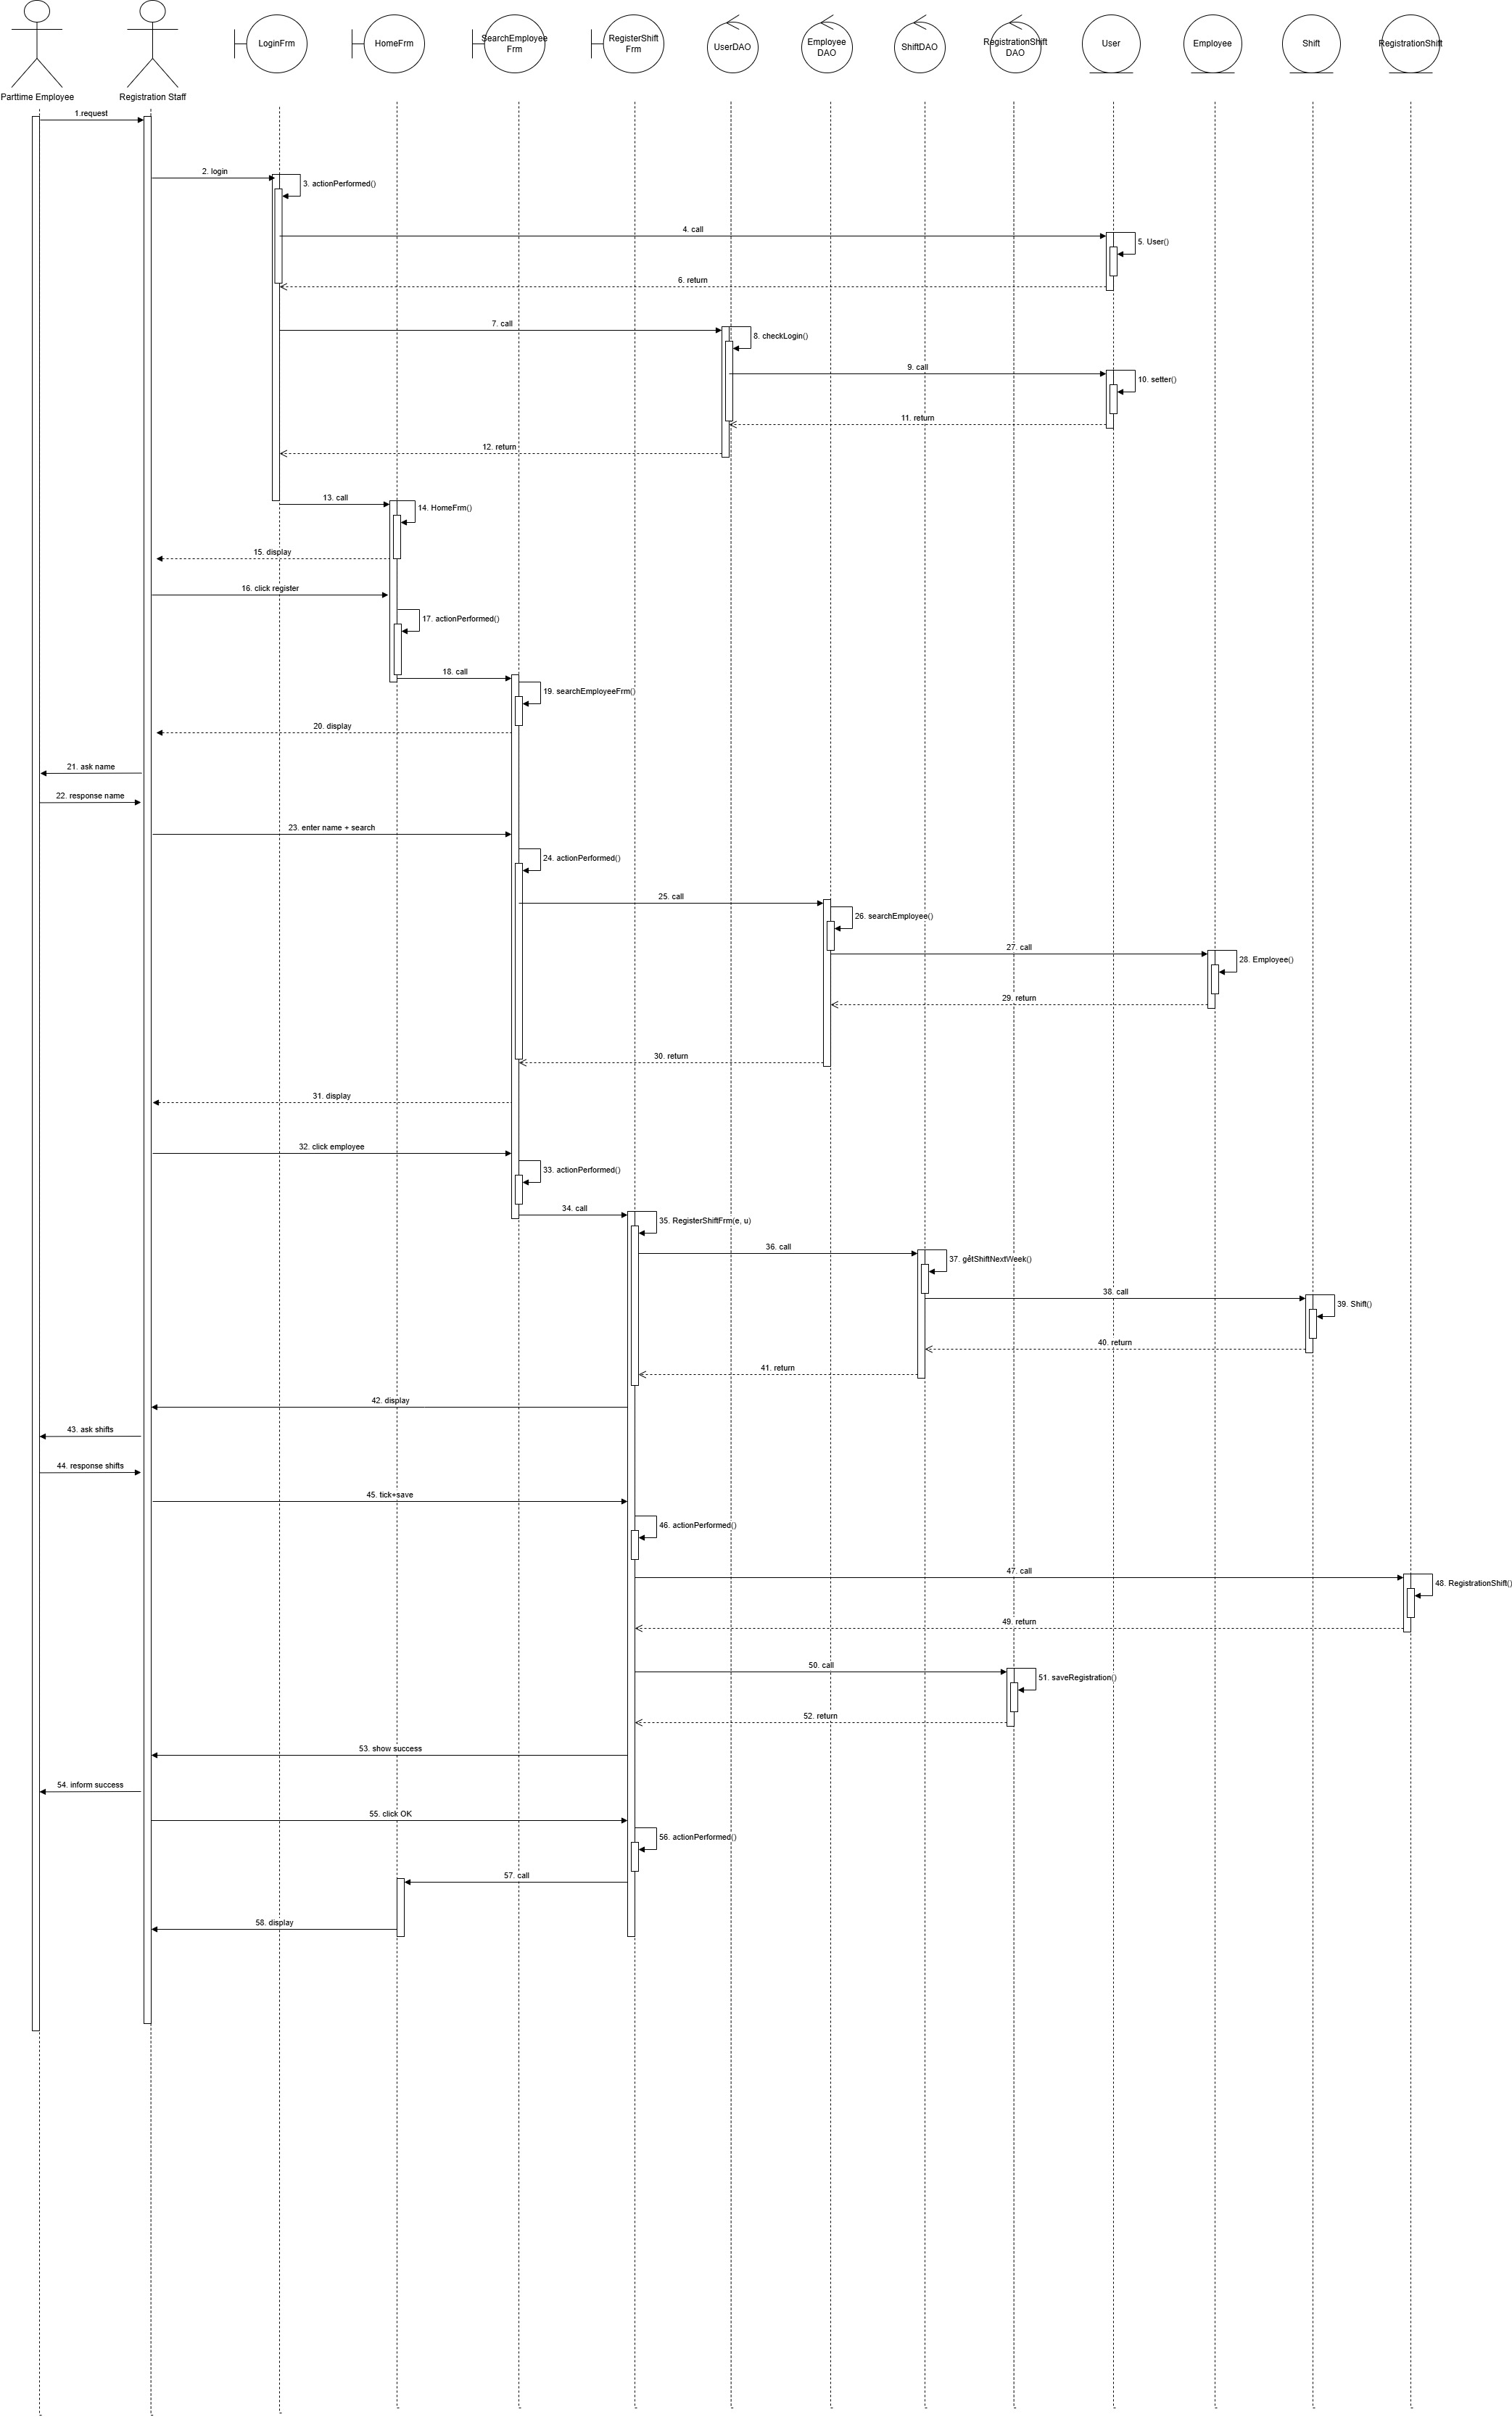
\includegraphics[width=0.95\textwidth]{assets/diagrams/Sequence Diagram Design.jpg}
    \caption{Sequence Diagram for the Standard Scenario in the Design Phase}
\end{figure}
